
\documentclass[12pt]{article} % Use A4 paper with a 12pt font size - different paper sizes will require manual recalculation of page margins and border positions

% Generated with LaTeXDraw 2.0.8
% Mon Jun 17 19:00:40 EDT 2013
\usepackage[usenames,dvipsnames]{pstricks}
\usepackage{epsfig}
\usepackage{pst-grad} % For gradients
\usepackage{pst-plot} % For axes
\usepackage[left=1.3cm,right=4.6cm,top=1.8cm,bottom=4.0cm,marginparwidth=3.4cm]{geometry} % Adjust page margins
\usepackage{amsmath} % Required for equation customization
\usepackage{amssymb} % Required to include mathematical symbols
\usepackage{xcolor} % Required to specify colors by name
\usepackage{amsthm}
\usepackage{float}
\usepackage{tikz}
\usetikzlibrary{shapes,backgrounds}
\usepackage{wasysym}
\date{}

\setlength{\parindent}{0cm} % Remove paragraph indentation
\newcommand{\tab}{\hspace*{2em}} % Defines a new command for some horizontal space


\title{Introduction to Probability Theory - Lecture 1}
%----------------------------------------------------------------------------------------

\newtheorem{defn}{Definition}
\newtheorem{example}{Example}
\newtheorem{prop}{Proposition}
\newtheorem{exer}{Exercises}
\newtheorem{thm}{Therorem}
\begin{document}
\maketitle
\section{Why do we study probability?}
Probability is the mathematical basis of the science of statistics. In particular, there are a couple of probability theorems that form the basis for much statistical inference: The Law of Large Numbers (LLN) and the Central Limit Theorem.\\

First, let's state an informal version of the LLN:\\

\begin{thm}
Let $X_1,...,X_n$ be independent samples from a population with mean $\mu$ (unknown) and define:
$$S_n = \frac{X_1+...+X_n}n$$.
Then as $n\rightarrow\infty, S_n\rightarrow\mu$.
\end{thm}
Question: in what sense does $S_n\rightarrow\mu$? What does this mean? What should it mean (intuitively)? 

Now, to really state the LLN, we need to be a bit more precise. \\
\begin{thm}
Let $X_1,...,X_n$ be independent and identically distributed random variables with mean $\mu$ and variance $\sigma^2<\infty$. Define:

$$S_n=\frac{X_1+...+X_n}{n}.$$

Then as $n\rightarrow\infty$, 

$$S_n\xrightarrow[a.s.]{p}\mu:$$
\end{thm}
The reason we state things formally is because formal statements are needed to prove theorems. Theorems are necessary to ensure we are not coming to erroneous conclusions (for example, the LLN stated above is for \emph{independent and identically distributed} random variables. We cannot come to the same conclusion if our variables are correlated or have different distributions (though there are extension theorems for those cases).

Now, lets have a quick look at a formal statement of the CLT:

\begin{thm}
Let $X_1,...,X_n$ be independent and identically distributed random variables with mean $\mu$ and variance $\sigma^2<\infty$. Define:

$$S_n=\frac{X_1+...+X_n}{n}.$$

Then as $n\rightarrow\infty$, 

$$\sqrt{n}\left(S_n-\mu\right)\xrightarrow{d} N(0,\sigma^2)$$
\end{thm}

In English, this means that the distribution of the fluctuations of the sample mean from the population mean $\mu$ approaches a normal distribution as $n$ gets large. The variance of the limiting normal distribution is the population variance.\\

Much of what we learn in this class will build the machinery to prove and fully understand these results. We won't cover the convergence part (that's in 704), but we will study random variables, distributions, independence, etc.\\

\section{What is Probability? - Naive Approach}
Now that we have (hopefully) agreed that probability is important to study, what exactly is it? We will begin with a 'naive' approach that is intuitive, but limited and then use what we have learned about the intuitive notion to define a theory of probability that is both more precise and more general.\\

We are going to need some terminology, so let's get that out of the way. When we talk about the probability of something happening, we usually mean as a result of some other thing happening. In other words, what is the probability of a coin landing heads up when tossed?\\

We call the coin toss an \emph{experiment} and the result an \emph{outcome}. An \emph{experiment} is some process of obtaining an observation of some phenomenon. A \emph{trial} is one iteration of an experiment. If our experiment is tossing a coin once, then tossing $10$ times would be $10$ trials.\\

Note: We could equally well define an experiment as tossing a coin 10 times. Then tossing it 100 times is ten trials. How we define the experiment depends on what we are interested in studying. \\

Finally, the \emph{set} of all outcomes is called the \emph{sample space}. This leads us on a slight detour - we'll need a tiny bit of set theory to proceed.

\subsection{A Detour via Set Theory}

A \emph{set} is simply a collection of objects. An object can be pretty much anything you can think of:

\begin{itemize}
\item $\left\{1,2,3,7,-5,-12\right\}$ - just a bunch of numbers
\item $\left\{2,4,6,8,...\right\}$ - even numbers
\item $\left\{\textrm{Dash, Bast, Tiberius (Gracchus), Chestnut}\right\}$ - my pets
\item $\left\{x:x>4\textrm{ and } x\in\mathbb{R}\right\}$ - all real numbers greater than 4
\end{itemize}

There are a few special sets:

\begin{itemize}
\item $\varnothing$ - the empty set. It's empty \smiley
\item $\Omega$ - the universal set. It contains \emph{everything}. In probability, the universal set is the sample space, usually denoted $S$.
\end{itemize}
\subsubsection{Subsets}
A subset is a set whose elements are \emph{all} contained in another set.\\\\
Example: If $A=\left\{1,2,3,4,5\right\}$, $B=\left\{1,2\right\}$ and $C=\left\{5,2,3\right\}$ and $D=\left\{5\right\}$, then $B,C$ and $D$ are all subsets of $A$ and $D$ is also a subset of $C$.\\

Formally: If $A$ and $B$ are sets, $B$ is a \emph{subset} of $A$ $\iff$ all elements of $B$ are also elements of $A$. If $B$ is a subset of $A$, we write:
$$B\subset A \textrm{ or } B\subseteq A$$ 
Some set facts:
\begin{itemize}
\item If $A$ is a set, $\varnothing\subset A$
\item If $A$ is a set $A\subset A$
\item  $A = B \iff A$ and $B$ are subsets of each other.\\
\end{itemize}
\subsubsection{Set Operations}
Sets are mathematical objects, and mathematical objects usually come with some 'operations' with which one may manipulate them. The following are some set operations (for $A$ and $B$ sets):

\begin{enumerate}
\item Union - denoted $A\cup B$. This is the set of all elements that are in $A$, together with all the elements that are in $B$.
\item Intersection - denoted $A\cap B$ This is the set of all elements that are in $A$ and also in $B$.
\item Complement - $A^c$ is the set of all elements of the universal set that are not contained in $A$.
\end{enumerate}
\def\firstcircle{(0,0) circle (1.5cm)}
\def\secondcircle{(0:2cm) circle (1.5cm)}
\def\bigcircle{(0:.5cm) circle (2.5 cm)}

% Now we can draw the sets:
\begin{tikzpicture}
%    \draw \firstcircle node[below] {$A$};
%    \draw \secondcircle node  {$B$};
%    \draw \thirdcircle node [below] {$C$};

    % We want to highlight the intersection of the first and the
    % second circle:
       \begin{scope}shift={(15cm,0cm)}
              \draw \firstcircle node[below] {$A$};
              \draw \secondcircle node  {$B$};
              \clip \firstcircle;
              \fill[red] \secondcircle;
              \draw \firstcircle node[below] {$A$};
              \draw \secondcircle node  {$B$};
              \draw (1,-2) node {bf{\huge{$A\cap B$}}};
                 \draw (1,-2) node {textcolor[black]{{\huge{$A\cap B$}}}};
          \end{scope}
       \draw (1,-2) node {$A\cap B$};

  \begin{scope}[shift={(-6cm,0cm)}]
          \begin{scope}[even odd rule]% first circle without the second
              \clip \secondcircle (-3,-3) rectangle (3,3);
          \fill[yellow] \firstcircle;
          \end{scope}
     % second circle without the first
               \fill[yellow] \secondcircle;
          \draw \firstcircle node {$A$};
          \draw \secondcircle node {$B$};
          \draw (1,-2) node {$A\cup B$};
      \end{scope}
      
    \begin{scope}[shift={(7cm,0cm)}]
             \begin{scope}[even odd rule]% first circle without the second
                 \clip  \firstcircle (-3,-3) rectangle (3,3);
             \fill[yellow] \bigcircle;
              
                          \draw \bigcircle node[below] {$S$};
                      
             \end{scope}
              \draw \firstcircle node {$A$};   
             \draw (1,-3) node {$A^c$};
             \draw (1,2) node {$S$};
        % second circle without the first
            
            
         \end{scope}
   
\end{tikzpicture}
\subsubsection{De Morgan's Laws}
De Morgan's laws are used often in probability proofs (because $P(A) = 1-P(A^c)$.\\

Suppose we would like to write $(A\cup B)^c$ in terms of an intersection. We know that  $(A\cup B)$ is everything in $A$ together with everything in $B$. That means $(A\cup B)^c$ is everything that is \emph{not} in $A$ \emph{and} everything that is \emph{not} in $B$. Mathematically, that means:
$$\left(A\cup B\right)^c = A^c\cap B^c$$

The analogous statement for intersections to unions is:
$$\left(A\cap B\right)^c = A^c\cup B^c$$

The result also holds for \emph{finite} unions and intersections, i.e. for $A_1,...,A_n$ sets :
$$\left(\bigcap_{i=1}^n A_i\right)^c = \bigcup_{i=1}^n A_i^c \textrm{ and } \left(\bigcup_{i=1}^n A_i\right)^c = \bigcap_{i=1}^n A_i^c$$
\subsubsection{Partitions}
We'll also make use of partitions quite a bit - especially with regards to something called the Law of Total Probability.\\
A \emph{partition} of a set $A$ is a collection $A_1,...,A_n$ of subsets of $A$ such that 
$$\bigcup_{i=1}^n A_i = A$$
and
$$A_i\cap A_j = \varnothing \textrm{ for } i\neq j$$
A partition of a set $A$ could look something like this:\\\\\\
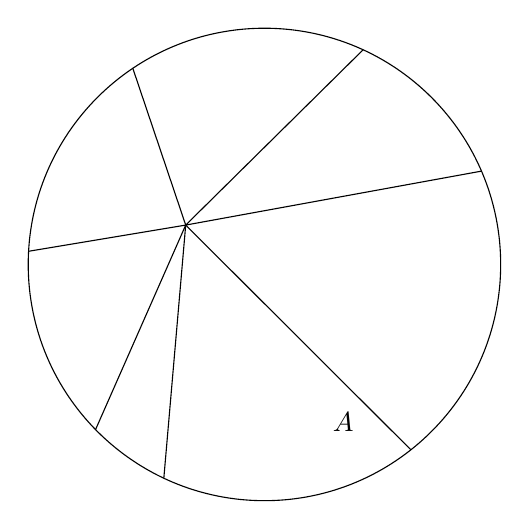
\begin{tikzpicture}
%    \draw \firstcircle node[below] {$A$};
%    \draw \secondcircle node  {$B$};
%    \draw \thirdcircle node [below] {$C$};

    % We want to highlight the intersection of the first and the
    % second circle:
       \begin{scope}shift={(15cm,0cm)}
            
              \draw[clip] (0,0) circle (3cm);
              \foreach \a in {20,60,120,180,230,250,310}
              {
              \draw (-1,.5) -- (\a:4cm);
              }
          \end{scope}
       \draw (1,-2) node {$A$};
\end{tikzpicture}
\subsubsection{Cardinality}
A property of sets that we are often interested in is their size. For finite sets, this is easy - the size or \emph{cardinality} of a finite set is the number of elements in that set. We denote the cardinality of a set $A$ by $|A|$.\\
 Things get a little trickier when we deal with infinite sets. Infinite sets may be \emph{countably infinite} or \emph{countable} or \emph{uncountable infinite} or \emph{uncountable}. As you might guess, a countable set is "smaller" than an uncountable set.\\
An infinite set is said to be \emph{countable} if its elements can be put in 1-1 correspondence with the set of natural numbers $\left\{0,1,2,3,...\right\}$. \\\\
Let's do this for the integers. We need take each of the elements of $\left\{...-3,-2,-1,0,1,2,3,...\right\}$ and assign it to one (and \emph{only} one) element of $\left\{0,1,2,3,...\right\}$. We do the following:
\begin{itemize}
\item Send $0 \in \left\{...-3,-2,-1,0,1,2,3,...\right\}$ to $0 \in \left\{0,1,2,3,...\right\}$
\item Send the negative numbers $\left\{-1,-2,-3,...\right\}$ to the odd numbers $\left\{1,3,5,...\right\}$ and the positive numbers $\left\{1,2,3,...\right\}$ to the even numbers $\left\{2,4,6,...\right\}$. And we are done!
\end{itemize}
So, we see th integers are countable. Sometimes, I may say a set is countable if it can be put in 1-1 correspondence with the integers. This is true - because any set that is in 1-1 correspondence with the natural numbers can be put in 1-1 correspondence with the integers, and vice-versa.\\
Lastly, we give an example of a set that is uncountable:
$$\left\{x\in\mathbb{R}:x>4\right\}$$
In English, this is read "$x$ in $\mathbb{R}$ (the real numbers), such that (the colon ':' is read as 'such that') $x$ is greater than $4$." Lest we think a set of real numbers must be unbounded to be uncountable, we also note that the set:
$$\left\{x\in \mathbb{R}: 0<x<1\right\}$$
is also uncountable. (Proofs of these results are beyond our scope - but any discrete math textbook will have one - or just look at Wikipedia.)

\subsection{More Definitions - Naive Probability}
\begin{defn}
The \emph{sample space} $S$ is the set of all possible outcomes of an experiment. Any subset $A\subset S$ is called an \emph{event}. We say that an even $A$ \emph{occurred} if the actual outcome is an element of $A$.
\end{defn}
\begin{example}
Consider a die roll and the following events:
$$A = \left\{1,3,5\right\}, B=\left\{6\right\}\textrm{ and } C=\left\{3\right\}$$
Suppose we roll the die and the result is a $3$. Then:
\begin{enumerate}
\item $A$ occurred
\item $C$ occurred
\item $A\cap C$ occurred
\item $B$ did not occur
\item $A\cup B$ occurred 
\end{enumerate}
\end{example}
Now, we are finally ready to set our naive definition of probability:
\begin{defn}
Let $S$ be a finite sample space and let $A$ be a subset of $S$. We define the function
$$P:S\rightarrow \left[ 0,1\right]$$
$$P(A) = \frac{|A|}{|S|}$$
where $|A|$ denotes the cardinality of the set $A$.
\end{defn}
Note: this definition has a couple of serious limitations:
\begin{enumerate}
\item It only works for finite sample spaces
\item It assumes that all outcomes are \emph{equally likely}.
\end{enumerate}
\end{document}